\section{Results and discussion}

\subsection{Calibration}

The values that have been found for $l_{real}$, $n$, $l_{pixel}$ and the corresponding error are presented in table \ref{table_pixelsize} for each objective. It was estimated that $u(n) = 4$.

The images corresponding to each measurement are presented in appendix \ref{appendix_calibration_4}, \ref{appendix_calibration_10} and \ref{appendix_calibration_40}.

\begin{table}[h!]
\label{table_pixelsize}

\centering
\captionsetup{font=small, justification = centering}
  \caption{Results of measurements of $n$ for the corresponding value of $l_{real}$ for each objective. The values for $l_{pixel}$ and $u(l_{pixel})$ follow from respectfully equation \ref{eq_pixelsize} and \ref{eq_u_pixelsize}.}

\begin{tabular}{|l|l|l|l|l|}
\hline

Objective & $l_{real} (m) \cdot 10^{-3}$ & $n$ & $l_{pixel}$ & $u(l_{pixel})$ \\ \hline
$4\times$ & 1 & 6.85$\cdot 10^2$ & 1.461$\cdot 10^{-6}$ & 9$\cdot 10^{-9}$\\
$10\times$ & 0.8 & 1.247$\cdot 10^3$ & 6.42$\cdot 10^{-7}$ & 2$\cdot 10^{-9}$ \\
$40\times$ & 0.2 & 1.250$\cdot 10^3$ & 1.600$\cdot 10^{-7}$ & 5$\cdot 10^{-10}$ \\ \hline
\end{tabular}
\end{table}


The values that have been found for $M_{A,B}$ for the different objective combinations are presented in table \ref{table_magnification}.

\begin{table}[h!]
\label{table_magnification}

\centering
\captionsetup{font=small, justification = centering}
  \caption{Calculated values for $M_{A,B}$ for the three different objective combinations.}

\begin{tabular}{|l|l|l|l|l|}
\hline

Objective A & Objective B & B/A & $M_{A,B}$ & $u(M_{A,B})$ \\ \hline
$\times 4$ & $\times 10$ & 2.5 & 2.28 & 2$\cdot 10^{-2}$\\
$\times 4$& $\times 40$ & 10 & 9.13 & 6$\cdot 10^{-2}$ \\
$\times 10$ & $\times 40$ & 4 & 4.01 & 2$\cdot 10^{-2}$ \\ \hline
\end{tabular}
\end{table}


As expected, the accuracy for the higher magnification objectives is better. Meaning that images from an objective with a higher magnification, corresponds with a smaller value for $l_{pixel}$. However, not all the values of $M_{A,B}$ match the theoretical relative magnification of $\frac{B}{A}$ taking into account the error.

since only the values of $M_{A,B}$ with $B = 40$ do not match the theoretical relative magnification, it would suggest that only the $\times 40$ objective is not true to its specifications. More research could be done to prove this with smaller uncertainty.

Apart from the fact that the objectives might not be true to specifications, this does not affect the results of this experiment. It proves, however, the importance of calibrating a microscopy set-up in order to get valid size measurements.

\bigskip


The values that have been found for $I_{max}$, $I_{min}$, $V_{is}$ and the corresponding errors are presented in table \ref{table_vis} in appendix \ref{appendix_vis_table}. In figure \ref{fig_vis_plot}, $V_{is}$ is plotted as a function of the spatial frequency for each objective. The images corresponding the measurements are presented in appendix \ref{appendix_vis_4}, \ref{appendix_vis_10} and \ref{appendix_vis_40}.

%plot_visibility

% Analysis

\subsection{Size measurements}

The values that have been found for $d_{hair}$ and $d_{gf}$ are respectively $d_{hair} =  $ and $d_{gf} =  $.

% analysis

The images used for this part of the experiment and the values that have been found for $a$, $b$, $A$ and the corresponding errors can be  in appendix \ref{appendix_starch}. A histogram of the values for $A$ is presented in figure \ref{fig_ellipse}.

% particle size histogram

% analysis

\subsection{Birefringence}

The colour planes that were taken into account for this experiment can be seen in figure \ref{fig_bf_planes} in which each Roman numeral corresponds to a colour plane.

% FIG_BF_PLANES

The values that have been found for $D$, $\delta d$ and the corresponding errors are presented in table \ref{table_bf} in appendix \ref{appendix_table_bf}.

In figure \ref{fig_bf_plot}, $\delta d$ is plotted as a function of $D$.

%BF PLOT

It follows from the orthogonal distance regression that $\delta n = XXX$.

%ANALYSIS






\subsection{Resolving power}
\begin{figure}[h!]
    \centering
    \begin{minipage}{.5\textwidth}
      \centering
      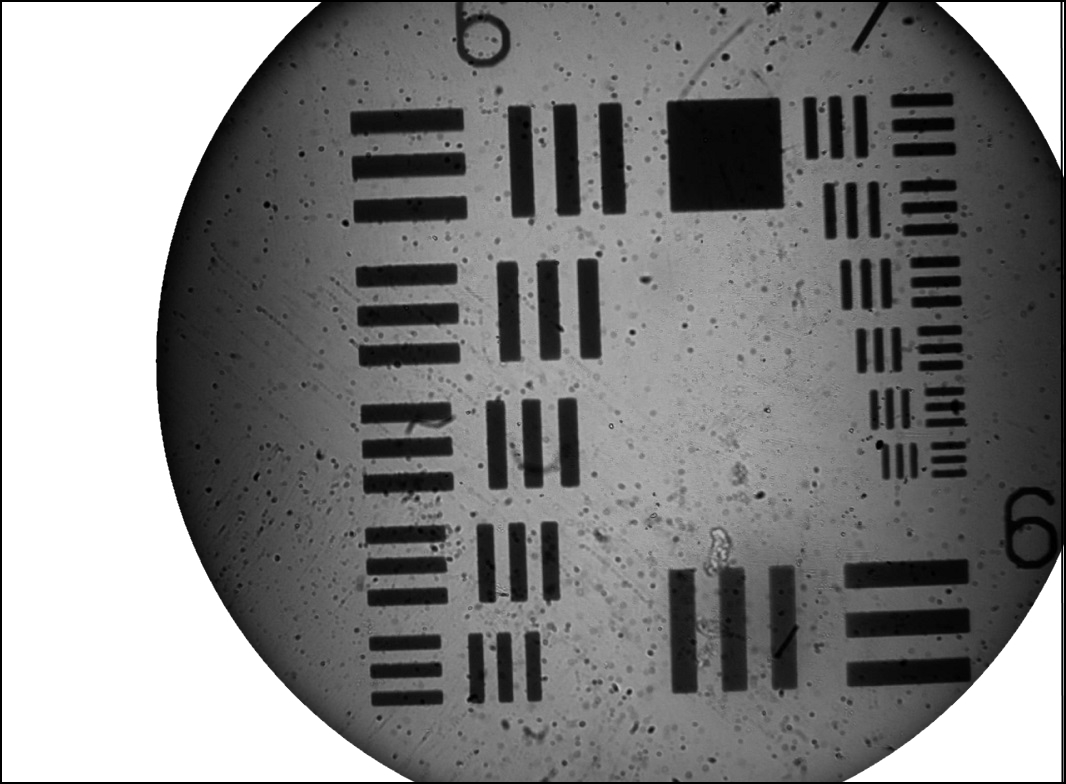
\includegraphics[width=0.7\textwidth,keepaspectratio]{afbeeldingen/process_visibility/m3_bw.jpg}
      \caption{Black and white photo.}
      \label{fig:resolution_target}
    \end{minipage}%
    \begin{minipage}{.5\textwidth}
      \centering
      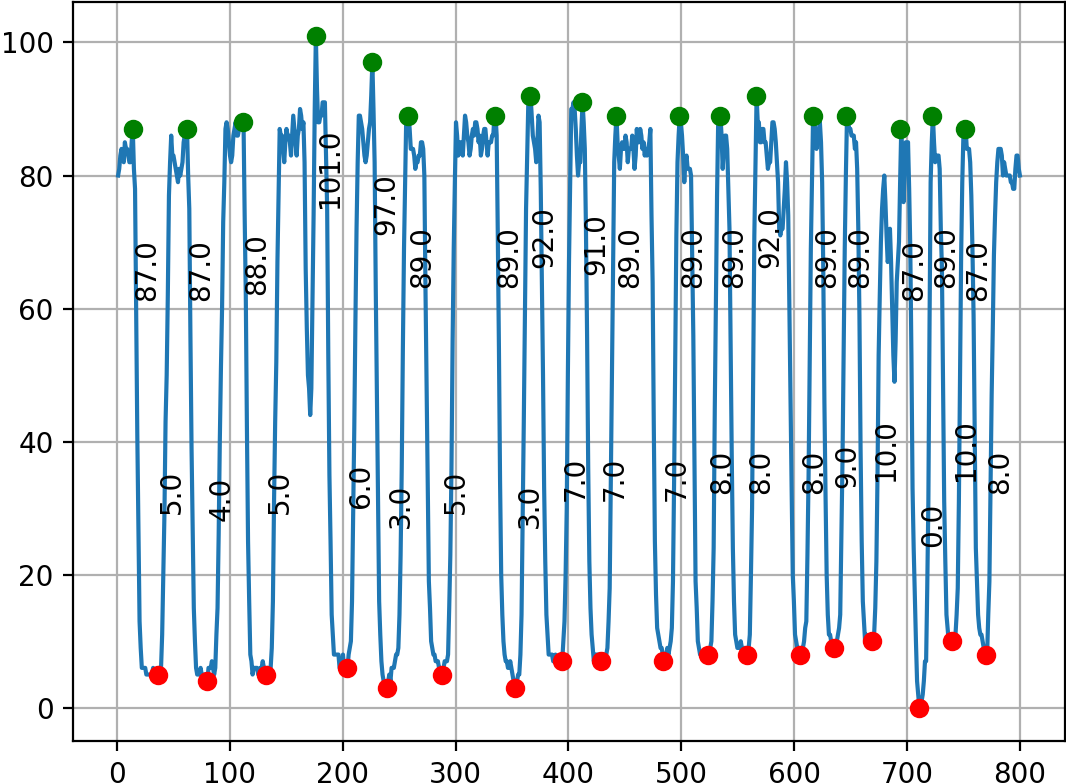
\includegraphics[width=0.7\textwidth,keepaspectratio]{afbeeldingen/process_visibility/m3_rpg_7.png}
      \caption{Linetrace of seventh group.}
      \label{fig:linetrace}
    \end{minipage}
\end{figure}

The above photos are the result of the process outlined in the previous section. The high an low values of the line trace were manually read of the photos and entered into a python script capable of calculating the visibility values for each magnification and spatial frequency. The result of which can be seen in figure \ref{fig:visibilities}.\\

\begin{wrapfigure}{l}{0.55\textwidth}
    \centering
    \vspace{-3mm}
    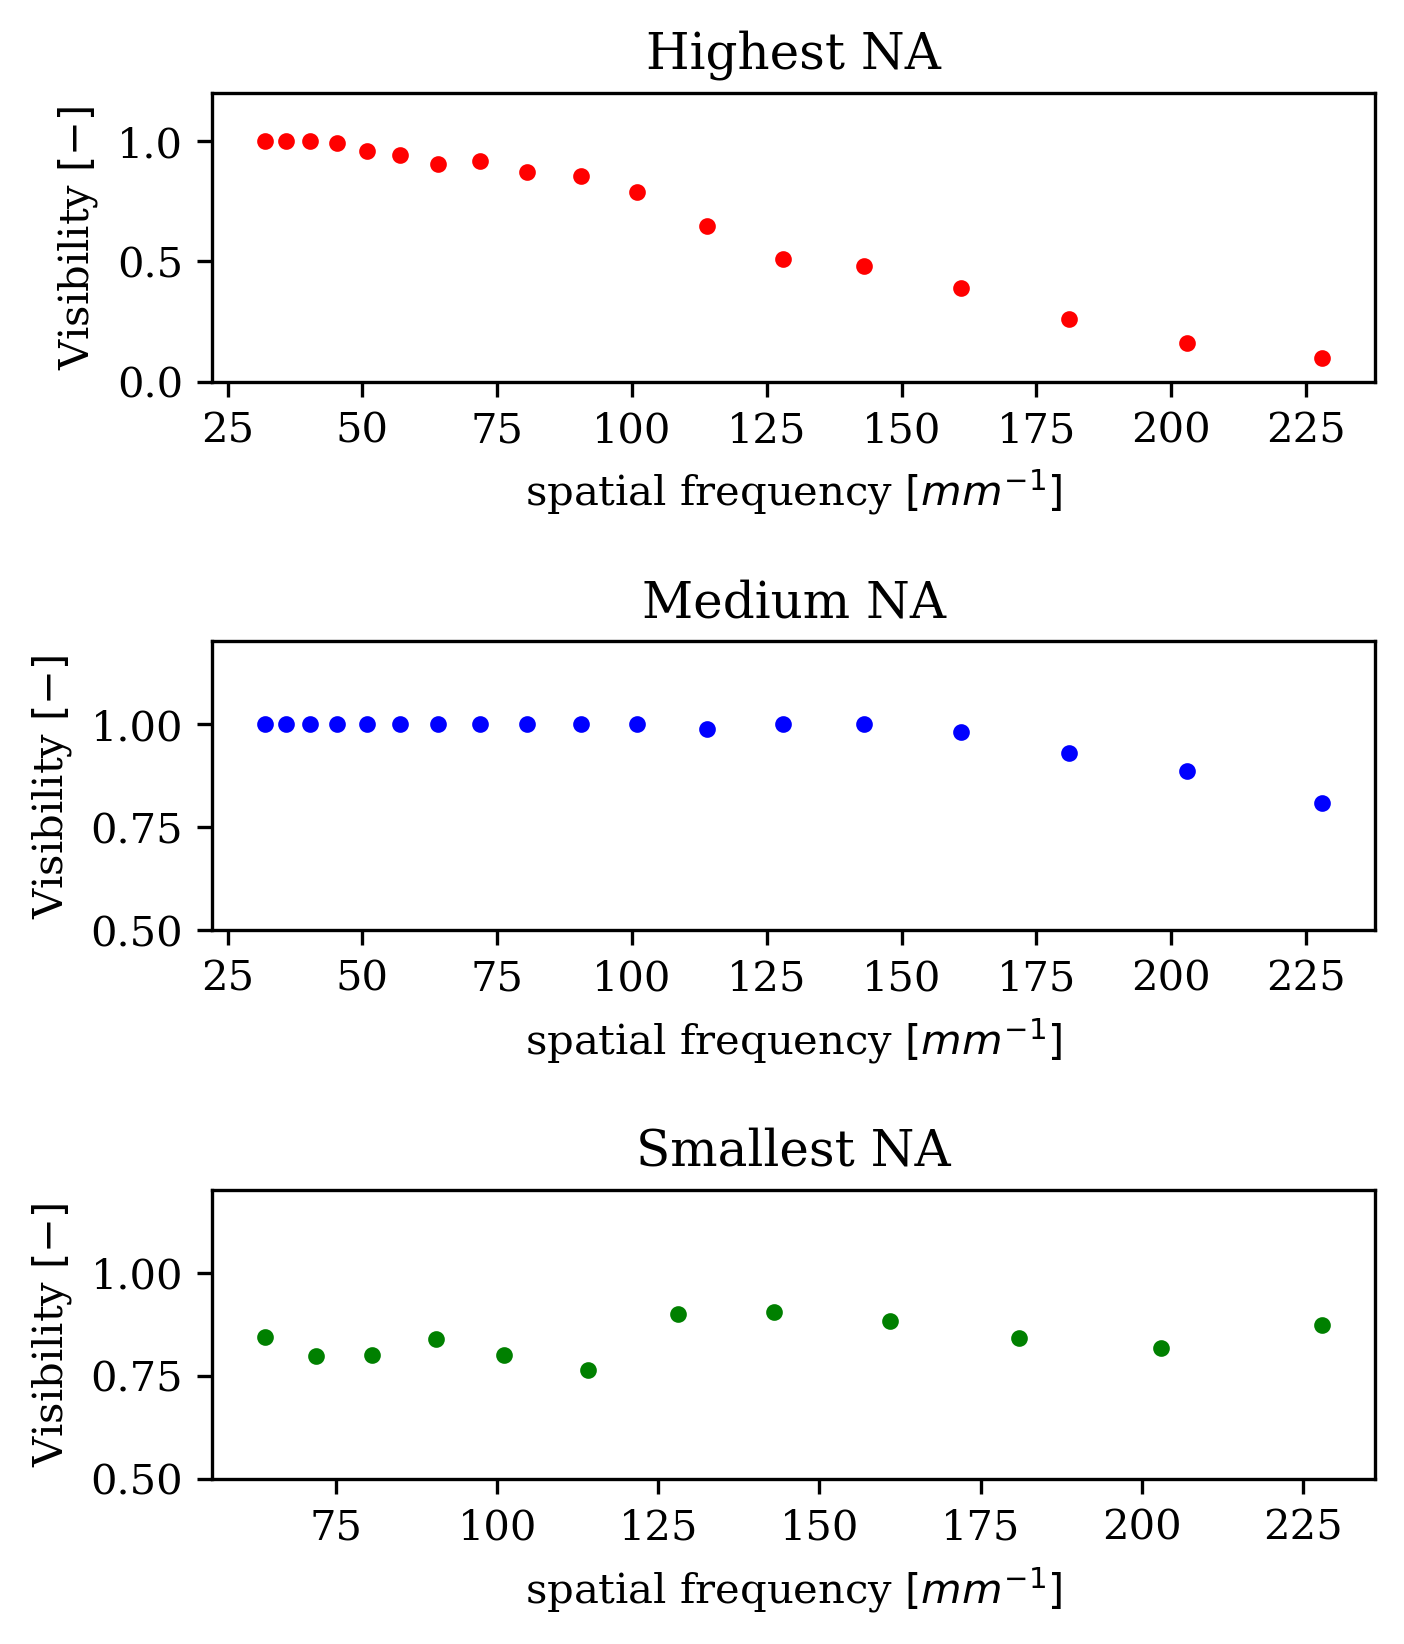
\includegraphics[width=0.55\textwidth,keepaspectratio]{afbeeldingen/visibilities.png}
    \caption{Plots of the visibilities per numerical aperature.}
    \label{fig:visibilities}
    \vspace{0mm}
\end{wrapfigure}

\vspace{-7mm}
The data is plotted in such a way that the highest subplot has the lowest magnification and the lowest subplot has the highest magnification. Each subplot has the dimensionless visibility number plotted on the vertical axis and the spatial frequency plotted on the horizontal axis. We chose this layout since we expect the visibility to decrease when the lines get closer together and the spatial frequency thusly increases. Note that only the verticle visibility axis of the highest subplot starts with a visibility of zero.\\
What we see is not surprising when we also take into account the photos in the appendix. As can be seen on these photos the highest magnification lense has the smallest numerical aperature, therefore all three traced groups are clearly resolvable. Thus the visibility won't drop as much as the lowest magnification lense when the spatial frequency increases.\\
Something noticable however is that the highest magnification plot starts of with the lowest visibility value. This has to do with the fact that this smaller aperature aslo catches less light, the brightest spot in its photo is evidently less bright than that of the other two aperatures. This can be seen when taking a look at either the linetraces or the photos in the appendix.


\begin{comment}
In theResultaten en discussie (Results and discussion) chapter, you present your results, generally in the form of graphs, and you discuss them. A single small table (m aximum ~10 rows x ~5 columns) is acceptable, but large tables should be in an appendix. In deviation from what many students believe, it is not desirable to separate the presentation and the discussion of results from each other. In professional literature, this is most often done together.\\ •You should introduce each graph:\\ -Why has this graph been included in the report. (What do we want to learn from this graph?).\\-Why   have   you   plotted   this   Y-axis   variable   as   a   function   of   this   X-axis   variable   (which   theoretical/expected relationship is tested/demonstrated in this this graph? \\•Then you tell the reader what (according to you) he/she should see in the graph, limiting yourself toconclusions  that  are  relatively  indisputable.  The  more  speculative  conclusions  should  be  in the  next  chapter.
\newpage
\end{comment}
